เราได้ผลการวิเคราะห์หาหัวข้อที่ผู้ใช้งานกล่าวถึงของโปรแกรม man man ดัง Table\ref{table:topicManMan} 
\begin{table}
	\caption{20 topic of man man application}
	\label{table:topicManMan}
	\centering
	\begin{tabular}{|l|r|
%			r|r|
		}
		\hline
		\multicolumn{1}{|c|}{topic} 
		& \multicolumn{1}{|c|}{sentiment} 
%		& \multicolumn{1}{|c|}{no. of positive} 
%		& \multicolumn{1}{|c|}{no. of negative}
		\\
		\hline
		{\selectlanguage{thai}เปลี่ยน ภาษา} & 0.2770 
%		& 35 & 9 
		\\
		\hline
		{\selectlanguage{thai}พัฒนา ยอด} & 0.2666 
%		& 47 & 6 
		\\
		\hline
		sticker {\selectlanguage{thai}หน่อย ขยาย} & 0.2046 
%		& 36 & 15 
		\\
		\hline
		{\selectlanguage{thai}สะดวก สวย} & 0.3926 
%		& 84 & 13 
		\\
		\hline
		{\selectlanguage{thai}สายตา ขนาด ใหญ่} & 0.5153 
%		& 143 & 26 
		\\
		\hline
		{\selectlanguage{thai}ยกเว้น ทำนาย} & 0.2315 
%		& 19 & 2 
		\\
		\hline
		{\selectlanguage{thai}ปรับปรุง ยาก} & 0.2035
%		 & 17 & 11 
		 \\
		\hline
		{\selectlanguage{thai}ปุ่ม หาย} & -0.5156 
%		& 49 & 23 
		\\
		\hline
		{\selectlanguage{thai}ชอบ แม่น} & 0.3926 
%		& 142 & 14 
		\\
		\hline
		{\selectlanguage{thai}สุดยอด ลอง} & 0.3926 
%		& 145 & 12 
		\\
		\hline
		{\selectlanguage{thai}แป้น รวน} & -0.3352 
%		& 24 & 9 
		\\
		\hline
		{\selectlanguage{thai}แก้ไข สี} & 0.2167 
%		& 40 & 15 
		\\
		\hline
		{\selectlanguage{thai}พิมพ์ ง่าย} & 0.5153 
%		& 201 & 12 
		\\
		\hline
		{\selectlanguage{thai}เสียง เสียดาย} & 0.4066
%		 & 17 & 4 
		 \\
		\hline
		{\selectlanguage{thai}ปรับ ขนาด ค้าง} & 0.5153 
%		& 63 & 13 
		\\
		\hline
		{\selectlanguage{thai}ปุ่ม แจ่ม ซับซ้อน} & -0.5156 
%		& 30 & 17 
		\\
		\hline
		{\selectlanguage{thai}เพิ่ม อิโมจิ} & 0.4066 
%		& 35 & 1 
		\\
		\hline
		{\selectlanguage{thai}เดา คำ} & -0.5156 
%		& 44 & 9 
		\\
		\hline
		{\selectlanguage{thai}พิมพ์ พลาด} & 0.5153 
%		& 68 & 11 
		\\
		\hline
		{\selectlanguage{thai}แป้น ใหญ่} & 0.3396 
%		& 82 & 13 
		\\
		\hline
	\end{tabular}
\end{table}
\begin{figure}
	\centering
	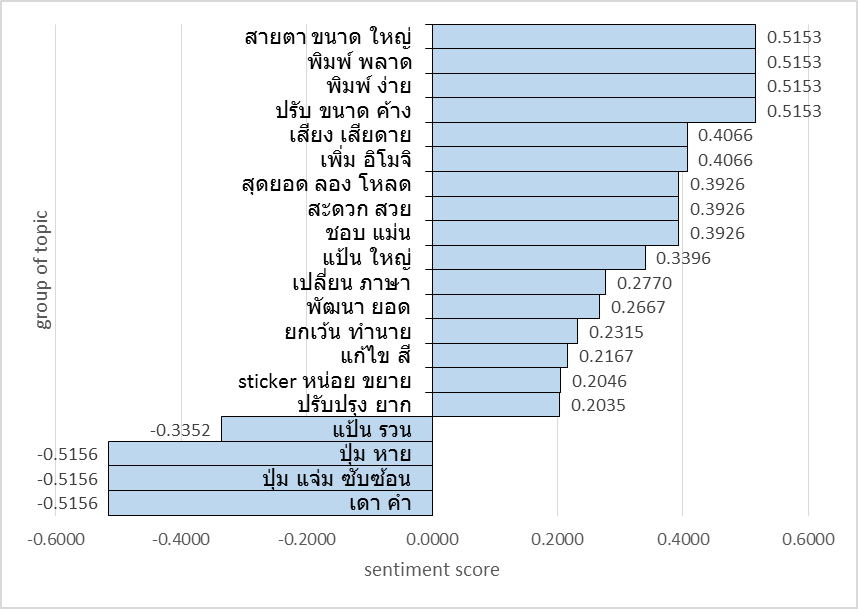
\includegraphics[width=0.9\linewidth]{graphmanman}
	\caption{sentiment score of topic from man man user reviews}
	\label{fig:graphmanman}
\end{figure}

โดยเราได้ตรวจสอบความถูกต้องของงานวิจัยโดยให้ผู้เชี่ยวชาญประเมินทัศนคติของประโยค ซึ่งจะได้ค่าความถูกต้องตาม Table \ref{table:f-measureSenti}
\begin{table}
	\caption{precision, recall, f-measure and accuracy for sentiment analysis}
	\label{table:f-measureSenti}
	\centering
	\begin{tabular}{|l|r|r|r|r|}
		\hline
		\multicolumn{1}{|c|}{\multirow{2}{*}{application}} &
		\multicolumn{4}{|c|}{Sentence}\\
		\cline{2-5}
		\multicolumn{1}{|c|}{}&
		\multicolumn{1}{|c|}{precision}&
		\multicolumn{1}{|c|}{recall}&
		\multicolumn{1}{|c|}{f-measure} &
		\multicolumn{1}{|c|}{accuracy} \\
		\hline
		Man Man & 0.5028 & 0.3189 & 0.3570 & 0.6110\\
		\hline
		H-Tv & 0.5208 & 0.2889 & 0.3366 & 0.4837 \\
		\hline
		K-mobile & 0.4535 & 0.2810 & 0.3240 & 0.5153 \\
		\hline
	\end{tabular}
\end{table}

%เพิ่มเติม
และความถูกต้องของทัศนคติของหัวข้อที่ผู้ใช้งานกล่าวถึงตาม Table\ref{table:f-measureTopic}
\begin{table}
	\caption{precision, recall, f-measure and accuracy for sentiment of topic}
	\label{table:f-measureTopic}
	\centering
	\begin{tabular}{|l|r|r|r|r|}
		\hline
		\multicolumn{1}{|c|}{\multirow{2}{*}{application}} & 
		\multicolumn{4}{|c|}{Topic} \\
		\cline{2-5}
		\multicolumn{1}{|c|}{} &
		\multicolumn{1}{|c|}{precision}&
		\multicolumn{1}{|c|}{recall}&
		\multicolumn{1}{|c|}{f-measure} &
		\multicolumn{1}{|c|}{accuracy} \\
		\hline
		Man Man & 0.7188 & 0.6538 & 0.6848 & 0.55\\
		\hline
		H-Tv & 0.5252 & 0.5333 & 0.5293 & 0.5\\
		\hline
		K-mobile & 0.2368 & 0.45 & 0.3103 & 0.45\\
		\hline
	\end{tabular}
\end{table}

%%%%%%%
โดยเรายังไม่ได้ทดสอบความถูกต้องในส่วนของการหากลุ่มของหัวข้อที่ผู้ใช้งานกล่าวถึง เนื่องจากการที่เราไม่สามารถกำหนดหัวข้อที่แน่นอน จึงเป็นปัญหาให้เกิดความลำบากในการจับกลุ่มของหัวข้อ เพราะแนวคิดการจับกลุ่มหัวข้อของแต่ละคนนั้นไม่เหมือนกัน ทำให้กลุ่มของหัวข้อของแต่ละคนที่ได้ออกมาอาจจะมีบางกลุ่มที่ไม่ตรงกันเลย หรือบางกลุ่มอาจจะผสมกัน เหมือนอย่างงานวิจัยของ Gunzmam and Laalej \cite{userslikefeature} ซึ่งมีปัญหาในการจัดกลุ่มของหัวข้อเช่นกัน

ดังนั้นเราจึงอนุมานว่า LDA ที่เราหาได้นั้นมีความถูกต้องในระดับหนึ่ง ซึ่งในภายภาคหน้าผู้วิจัยจะพยายามหาวิธีการวัดความถูกต้องของการจับกลุ่มหัวข้อที่ไม่แน่นอนนี้ให้ได้

%%%%%%%


%%

\subsection*{Limitation}
เนื่องจากเรายังหาวิธีที่จะใช้ในการแบ่งประโยคที่ชัดเจนยังไม่ได้จึงทำให้การแบ่งประโยคนั้นอาจยังไม่ถูกต้อง รวมถึงคำบางคำ อาจจะเป็นคำสมัยใหม่ หรือภาษาวัยรุ่น ทำให้คำเหล่านี้ไม่มีอยู่ใน corpus ที่เราใช้งาน จึงเป็นเหตุให้เราอาจไม่สามารถหาทัศนคติของคำเหล่านี้ได้

และในการหา sentiment โดยการแปลภาษาไทย-อังกฤษ คำบางที่แปลได้ อาจแปลได้ไม่ตรงตามความต้องการของประโยคทั้งนี้เนื่องมาจาก การหา POS และ การพ้องรูปในภาษาไทย

อีกทั้งในเรื่องของการหาหัวข้อที่ไม่มีความแน่นอนของโปรแกรมต่าง ๆ จึงทำให้เรากำหนดจำนวนหัวข้อที่ต้องการไม่ได้



% An example of a double column floating figure using two subfigures.
% (The subfig.sty package must be loaded for this to work.)
% The subfigure \label commands are set within each subfloat command,
% and the \label for the overall figure must come after \caption.
% \hfil is used as a separator to get equal spacing.
% Watch out that the combined width of all the subfigures on a 
% line do not exceed the text width or a line break will occur.
%
%\begin{figure*}[!t]
%\centering
%\subfloat[Case I]{\includegraphics[width=2.5in]{box}%
%\label{fig_first_case}}
%\hfil
%\subfloat[Case II]{\includegraphics[width=2.5in]{box}%
%\label{fig_second_case}}
%\caption{Simulation results for the network.}
%\label{fig_sim}
%\end{figure*}
%
% Note that often IEEE papers with subfigures do not employ subfigure
% captions (using the optional argument to \subfloat[]), but instead will
% reference/describe all of them (a), (b), etc., within the main caption.
% Be aware that for subfig.sty to generate the (a), (b), etc., subfigure
% labels, the optional argument to \subfloat must be present. If a
% subcaption is not desired, just leave its contents blank,
% e.g., \subfloat[].


% An example of a floating table. Note that, for IEEE style tables, the
% \caption command should come BEFORE the table and, given that table
% captions serve much like titles, are usually capitalized except for words
% such as a, an, and, as, at, but, by, for, in, nor, of, on, or, the, to
% and up, which are usually not capitalized unless they are the first or
% last word of the caption. Table text will default to \footnotesize as
% the IEEE normally uses this smaller font for tables.
% The \label must come after \caption as always.
%
%\begin{table}[!t]
%% increase table row spacing, adjust to taste
%\renewcommand{\arraystretch}{1.3}
% if using array.sty, it might be a good idea to tweak the value of
% \extrarowheight as needed to properly center the text within the cells
%\caption{An Example of a Table}
%\label{table_example}
%\centering
%% Some packages, such as MDW tools, offer better commands for making tables
%% than the plain LaTeX2e tabular which is used here.
%\begin{tabular}{|c||c|}
%\hline
%One & Two\\
%\hline
%Three & Four\\
%\hline
%\end{tabular}
%\end{table}


%\begin{table*}[h]
%	\caption{example of result after pass POS tagger process}
%	\label{table:POSEx}
%	\centering
%	\begin{tabular}{|l|l|l|}
%		\hline
%		\multicolumn{1}{|c|}{sentense} &
%		\multicolumn{1}{|c|}{word segmentation} &
%		\multicolumn{1}{|c|}{POS}\\
%		\hline
%		ใช้ได้ดีครับ & 
%		ใช้ได้|ดี|ครับ| & 
%		ใช้ได้/npn ดี/vi ครับ/aff \\
%		\hline
%		เยี่ยม ดี เลิศ & 
%		เยี่ยม|ดี|เลิศ| & 
%		เยี่ยม/vt ดี/adv เลิศ/adv \\
%		\hline
%		พักหลังนี่อัพบ่อยนะครับ & 
%		พัก|หลัง|นี่|อัพบ่อย|นะ|ครับ| & 
%		พัก/vi หลัง/adj นี่/pdem อัพบ่อย/npn นะ/part ครับ/aff \\
%		\hline
%		ชอบค่ะใช้ง่าย มีตัวการ์ตูนให้ด้วย & 
%		ชอบ|ค่ะ|ใช้|ง่าย|มี|ตัว|การ์ตูน|ให้|ด้วย| & 
%		ชอบ/vt ค่ะ/aff ใช้/vt ง่าย/adv มี/vt ตัว/ncn การ์ตูน/ncn ให้/vpost ด้วย/adv \\
%		\hline
%		เรียบง่ายแต่ใช้ได้ดีจริงๆครับชอบมาก & 
%		เรียบง่าย|แต่|ใช้ได้|ดี|จริงๆ|ครับ|ชอบมาก| & 
%		เรียบง่าย/vi แต่/conj ใช้ได้/npn ดี/vi จริงๆ/adv ครับ/aff ชอบ/vt มาก/adv \\
%		\hline
%		ดีมากครับ สะดวกดีแม่นสุดยอด & 
%		ดีมาก|ครับ|สะดวก|ดี|แม่น|สุดยอด| & 
%		ดีมาก/npn ครับ/aff สะดวก/vi ดี/adv แม่น/vt สุดยอด/adj \\
%		\hline
%	\end{tabular}
%\end{table*}


